\chapter{Grundlagen}

\section{Historie}

Seit dem Beginn des Industriezeitalters um 1800, welches mit der Mechanisierung (Industrie 1.0) startete, befindet sich die Industrie in einem stetigen Wandel. Sie entwickelte sich um 1900 durch die Massenproduktion zur Industrie 2.0 und in den 1970er Jahren durch die Automatisierung zur Industrie 3.0. Die Einteilung der Industriezeitalter ist durch tiefgreifende Veränderungen im technologischen Fortschritt möglich, welche auch als industrielle Revolution bezeichnet werden. Aktuell befinden wir uns in der Phase der 4. industriellen Revolution.

\subsection{1. industrielle Revolution}

Die 1. industrielle Revolution fand mit der Erfindung der Dampfmaschine statt. Sie ermöglichte es Eisenbahnen und Dampfschiffe sowie verschiedene Maschinen im Kohleabbau oder in Textilfabriken anzutreiben und trug massiv zur Industrialisierung und der Entstehung der Industrie 1.0 bei. Nach und nach wurden immer mehr Produktionsanlagen errichtet und somit Arbeitsplätze in Infrastruktur, Textilfabriken, Häuserbau, Kohleabbau und anderen Bereichen geschaffen.

\subsection{2. industrielle Revolution}

Die Erforschung der Elektrizität im 19. Jahrhundert war der Auslöser der 2. industriellen Revolution. Nachdem ab 1830 die Gesetze der Elektrotechnik bekannt waren, fand die Elektrizität eine breite Anwendung in der Industrie und im Alltag. Im Jahr 1913 führte Henry Ford das Fließband in der Automobilbranche ein. Im Zuge dessen musste jeder Arbeiter nur noch einen Arbeitsschritt erledigen, welches einerseits die Produktion wesentlich beschleunigte und eine Massenproduktion ermöglichte und andererseits eine hohe Spezialisierung der einzelnen Arbeitskräfte für ihre bestimmte Aufgabe erforderte.

Außerdem wurde es durch die Luftfahrt möglich Produkte wie Autos, Kleidung und Lebensmittel über Kontinente hinweg immer schneller zu transportieren und zu handeln.

\subsection{3. industrielle Revolution}

Die 3. industrielle Revolution fand in den 1970er Jahren statt. Sie ist durch eine sukzessive (Teil-) Automatisierung der Prozesse und durch den Einzug der IT in die Industrie- und Verbraucherwelt geprägt. In den 1940er Jahren wurden die ersten Rechenmaschinen und programmierbare Steuerungen in Unternehmen eingesetzt. In den 1970er Jahren zog der Computer auch in den Privatbereich ein, wurde zunehmend beliebter und schaffte einen neuen Industriezweig. Der Fertigungsprozess in Fabriken wurde mehr und mehr von Maschinen übernommen.

Durch den zunehmenden Einsatz von IT in Unternehmen entstand immer mehr Kommunikation zwischen Menschen und Maschinenn. Diese Kommunikation und die anfallenden Daten wurden jedoch nur unternehmensintern verarbeitet. Es gab nur wenige Schnittstellen nach außen.

\begin{figure}[h]
  \centering
  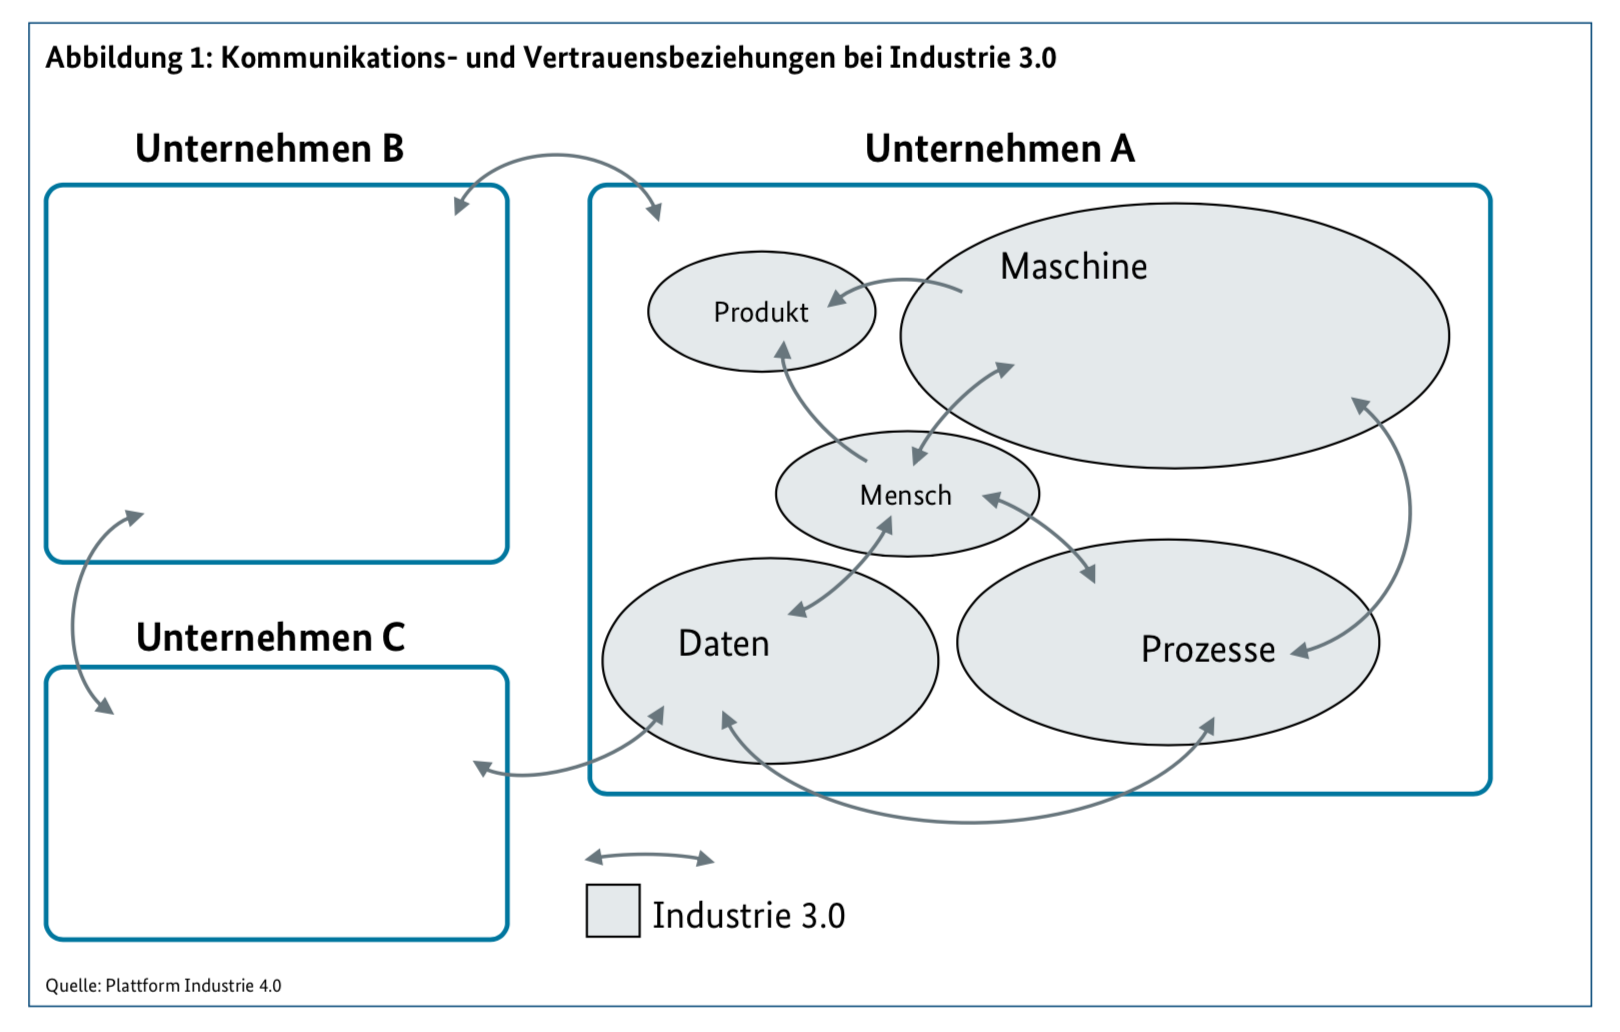
\includegraphics[width=15cm]{kommunikationsbeziehungen-i30}
  \caption{Kommunikationsbeziehungen in einer Industrie 3.0 Umgebung - TODO ref. sichere unternehmensübergreifende Kommunikation}
  \label{Kap2:Industrie3.0-Kommunikation}
\end{figure}

\clearpage

\subsection{4. industrielle Revolution}

Das Ende des 20. Jahrhunderts gilt als der Beginn der 4. industriellen Revolution. Das Kennzeichen dieser Phase ist die zunehmende Digitalisierung. Mit ihr geht die technische Vernetzung physischer Gegenstände, dem \ac{IOT}, einher. Mehr und mehr Geräte oder Gegenstände besitzen die Möglichkeit aktiv durch Datenaustausch oder passiv z. B. mit Hilfe eines Bar- oder QR-Codes mit der digitalen Welt zu kommunizieren und somit eine fortschreitende Automatisierung sowie Individualisierung zu ermöglichen. 

Im Gegensatz zur Industrie 3.0 sollen Maschinen autonom, auch über Unternehmensgrenzen hinweg, miteinander kommunizieren können um gesamte Geschäftsprozesse zu übernehmen. Dies setzt eine Öffnung der Unternehmen nach außen voraus.

\begin{figure}[h]
  \centering
  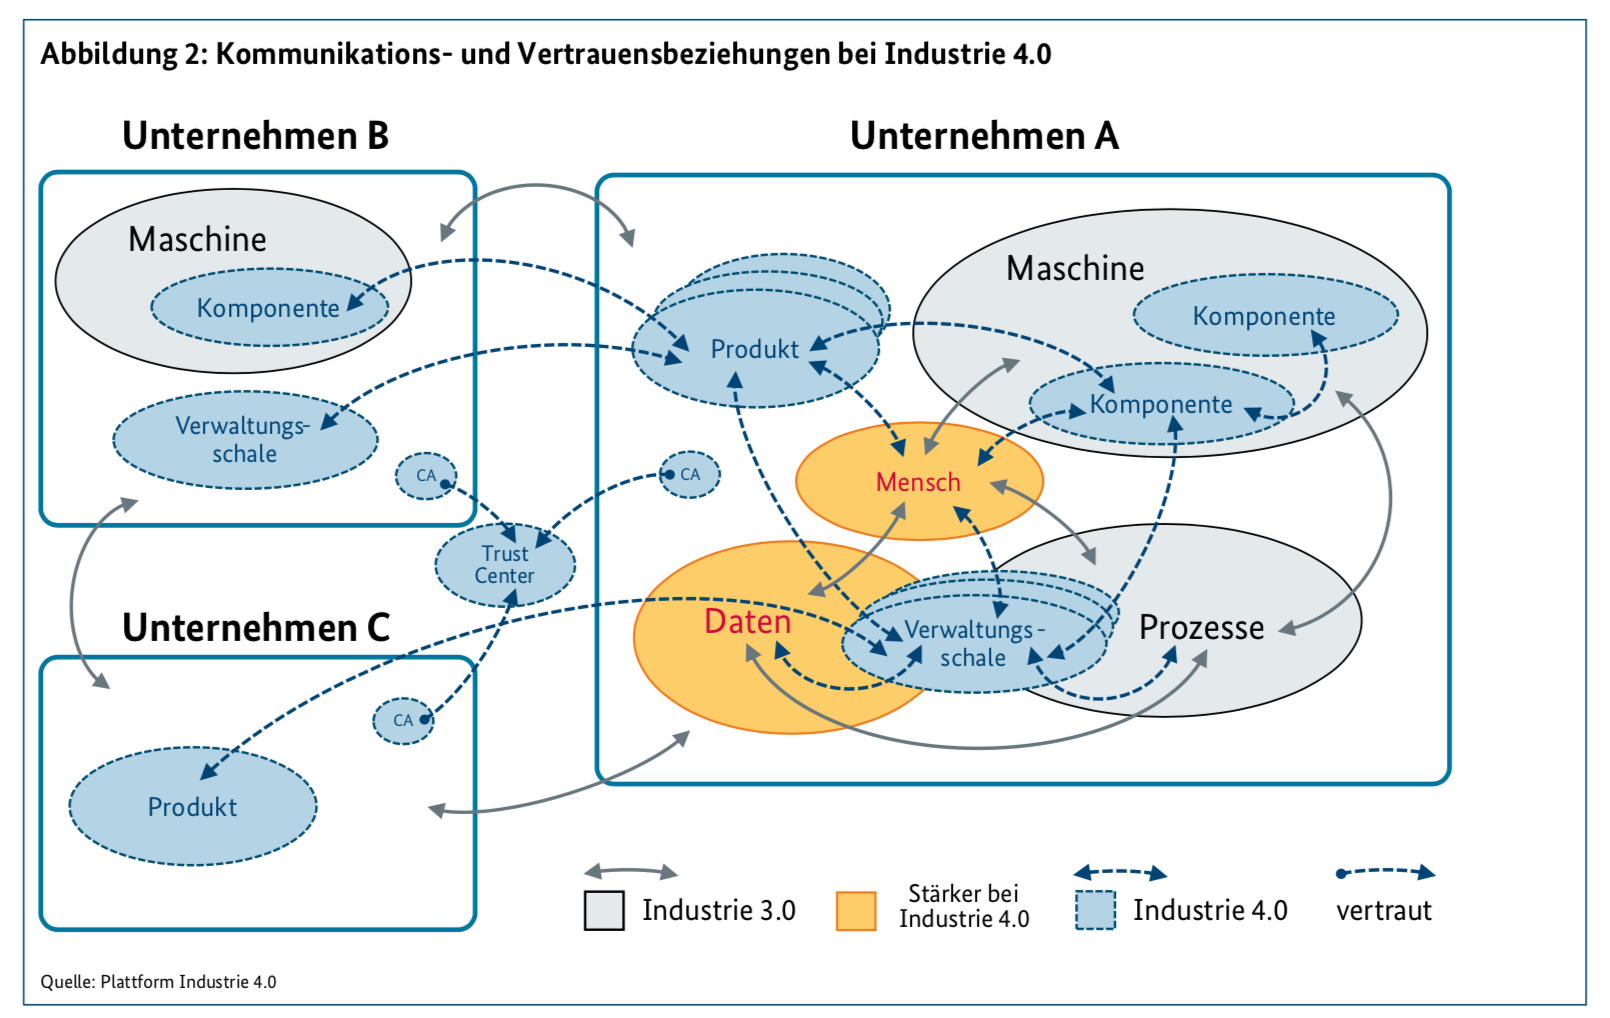
\includegraphics[width=15cm]{kommunikationsbeziehungen-i40}
  \caption{Kommunikationsbeziehungen in einer Industrie 4.0 Umgebung - TODO ref. sichere Unternehmensübergreifende Kommunikation}
  \label{Kap2:Industrie4.0-Kommunikation}
\end{figure}

\clearpage

Diese Entwicklung erzeugt durch die ständige Kommunikation eine ernome Menge an Daten, welche den Anforderungen der IT-Sicherheit gerecht werden müssen, um Verbraucher und Unternehmen zu schützen.

\section{aktueller Stand der Technik}
Der Prozess der vierten industriellen Revolution ist ein stetiger, nicht abgeschlossener Prozess. Aktuell werden die ersten Smart Factories der Industrie errichtet und erste smarte Einkaufsmöglichkeiten, wie Amazon Go und TODO - siehe Trumpf, für den Endverbraucher geschaffen. Diese Fabriken und Filialen stellen die ersten ihrer Art dar und dienen als Prototypen. Das Ziel des Wandels in der Strukturierung und Organisation der Produktion in Unternehmen ist eine immer weitere Automatisierung der Prozessabwicklung bis hin zu autonom arbeitenden Fabriken.

TODO - Trumpf

Die Umsetzung dieser Innovationen basiert hauptsächlich auf dem Fortschritt der \ac{IT} und dem Einzug der Internet-Technologien in die Industrie. Diese Entwicklung macht es möglich immer schneller Informationen auszutauschen, größere Datenmengen zu analysieren und diese zu verarbeiten. In der Industrie entstehen dadurch u. a. die folgenden Chancen:

\begin{itemize}
  \item Die Kommunikationsinfrastruktur wird in Zukunft in Produktionssystemen so preiswert sein, dass sie sinnvoll für Konfiguration, Service, Diagnose, Bedienung und Wartung genutzt werden kann.
  \item Die Produktionssysteme werden mehr und mehr mit einem Netz verbunden, erhalten dort eine digitale Identität, werden somit such- und analysierbar und besitzen die Möglichkeit Daten über sich selbst zu veröffentlichen. 
  \item Maschinen und Anlagen speichern ihre Zustände in ihrer digitalen Identität im Netz. Diese Zustände sind aktuell, aktualisierbar und zunehmend vollständig. Sind im Netzwerk viele solcher Identitäten vorhanden, können die Daten effizient abgerufen und ausgetauscht werden.
  \item Softwaredienste werden über das Netz verknüpft werden und können somit automatisiert individuelle Aufgaben durch die direkte Kommunikation der Systeme erledigen. Eine solche individuelle Wertschöpfung war bisher nur unwirtschaftlich oder gar nicht möglich.
\end{itemize}

Diese Veränderungen im Wertschöpfungsprozess und die ständige Kommunikation der Systeme bereiten jedoch auch Probleme. Es entstehen große Mengen an Daten, welche u. a. über einen unsicheren Kanal verbreitet werden sollen. Des weiteren sind viele vorhandene Produktionsanlagen nicht für diese Form von vermaschter Kommunikation entwickelt worden. Diesen Problemen wird aktuell durch die Entwicklung von Industriestandards und \ac{M2M}-Protokollen, wie z. B. die \ac{OPC UA} entgegengewirkt. Um vorhandene Anlagen weiterhin nutzen zu können, werden Gateways genutzt. (TODO Trumpf ref.)

\section{Industrie 4.0}

Der Begriff Industrie 4.0 wurde erstmals auf der Hannover Messe 2011 verwendet (\cite{drath2014}) und soll das Ergebnis der 4. industriellen Revolution darstellen. Der Grundgedanke hinter Industrie 4.0 ist die flächendeckende Vernetzung von Informations- und Kommunikationstechnik zu einem Internet der Dinge, Dienste und Daten (\cite{Spath2013}). Diese Vernetzung soll einen ständigen Informationsaustausch zwischen den Komponenten ermöglichen. Jede Komponente des \ac{IOT} soll als \ac{CPS} arbeiten. Ein \ac{CPS} besitzt neben seiner realen Identität eine digitale Identität, über welche es ständig mit anderen \ac{IOT}-Geräten kommunizieren kann. Kunden- und Maschinendaten werden miteinander vernetzt \cite{rami2016}.

\begin{figure}[h]
  \centering
  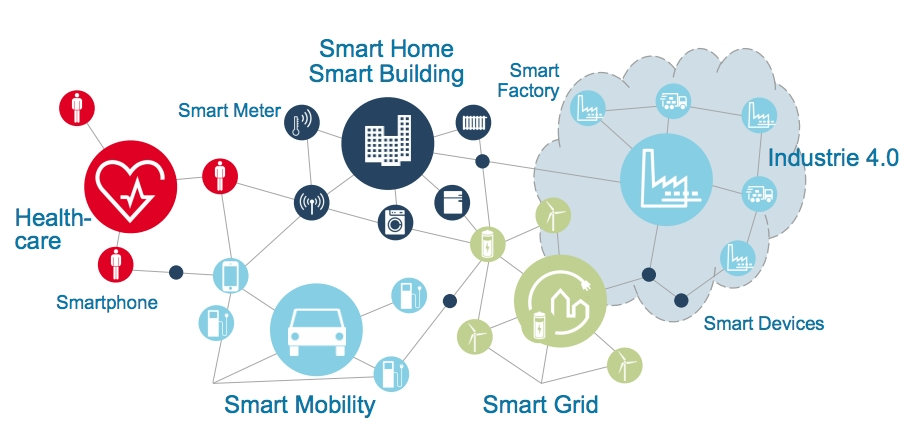
\includegraphics[width=15cm]{internet-der-dinge}
  \caption{Das Internet der Dinge - \cite{rami2016}}
  \label{Kap2:Das Internet der Dinge}
\end{figure}

\clearpage

Für Unternehmen bedeutet dies einen Wechsel von einer linearen Prozesskette hin zu einem vermaschten Netzwerk, in dem jede Komponente mit dem gesamten Netzwerk kommunizieren kann. Dies beinhaltet die Vernetzung der Komponenten auf horizontaler und vertikaler Ebene. Die vertikale Ebene stellt die technischen Komponenten dar und wird durch die Automatisierungspyramide beschrieben. Die horizontale Ebene beschreibt die wirtschaftlichen Geschäfts- bzw. Produktionsprozesse und besteht u. a. aus: Einkauf, Lieferanten, Produktionsplanung, Logistik, Sequenzierung und Lagerverwaltung. Das Ziel ist die Vernetzung aller Beteiligten.

\begin{figure}[h]
  \centering
  \includegraphics[width=15cm]{horizontaleVertikaleIntegration}
  \caption{horizontale und vertikale Integration - TODO ref. HP industry-of-things siehe bookmark}
  \label{Kap2:horizontale und vertikale Integration}
\end{figure}

\clearpage

TODO - nur Kommunikation auf vertikaler Achse untersucht

\subsection{Automatisierungspyramide}
Die Automatisierungspyramide stellt die beteiligten Systeme und Softwarekomponenten eines automatisierten Prozesses systematisch dar. Diese beginnen, ausgehend vom Kundenauftrag und der betriebswirtschaftlichen Planung der Produktion auf der Unternehmensebene im \ac{ERP} System. Die Ergebnisse der Planung werden an das \ac{MES} übergeben, welches die verschiedenen Fertigungs- oder Logistikaufträge generiert. Die Aufträge werden anschließend auf der Prozessleit- (\ac{SCADA}), Steuerungs- (\ac{SPS}) und Feldebene (Ein-/Ausgangssignale) bearbeitet.

\begin{figure}[h]
  \centering
  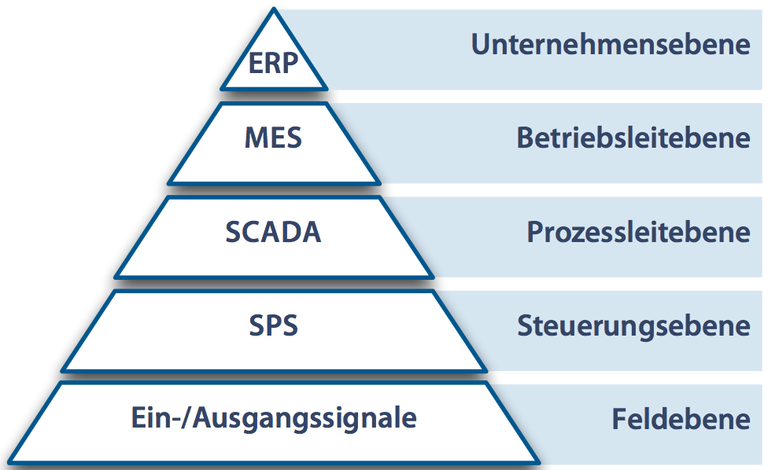
\includegraphics[width=10cm]{automatisierungspyramide}
  \caption{Automatisierungspyramide - TODO ref. Langmann,2004}
  \label{Kap2:Automatisierungspyramide}
\end{figure}

\clearpage

Während die oberen Schichten der Pyramide (\ac{ERP} und \ac{MES}) durch Standardkomponenten bzw. -software der IT realisiert werden, zählen die unteren Schichten (Prozessleit- bis Feldebene) zur Automatisierung, welche die Steuerung und Kontrolle der technischen Anlagen übernimmt. Diese werden auch als Shop-Floor-Ebene bezeichnet. Sie sind durch spezielle Hard- und Softwarelösungen umgesetzt. Die Kommunikation dieser Systeme ist u. a. für spezielle Anwendungsfälle wie harte Echtzeitreaktionszeiten mit Verzögerungen <1ms ausgelegt. Die Integration von Sicherheitsmaßnahmen bei der Kommunikation dieser Systeme stellt oft eine große Herausforderung dar.

\subsection{\ac{RAMI4.0}}
Um eine flächendeckende Vernetzung zu ermöglichen, muss eine einheitliche Kommunikation geschaffen werden. Die \ac{RAMI4.0} ist eine dreidimensionale Darstellung aller Teilnehmer einer Industrie 4.0 Umgebung und stellt ein Modell einer serviceorientierten Architektur dar. Sie soll eine Verwaltungsschale für Teilnehmer bilden, um eine standardisierte Kommunikation und einfache Inbetriebnahme neuer Komponenten ermöglichen. \cite{rami2016} Die Achsen der \ac{RAMI4.0} bestehen aus:

\begin{itemize}
  \item Achse 1 - Die Hierarchie zeigt die Anlagen, Maschinen sowie das Endprodukt, welche miteinander Vernetzt sind. In diesem Netzwerk werden Funktionen bereitgestellt und Daten ausgetauscht.
  \item Achse 2 - Architektur: 
  \item Achse 3 - Der Produktlebenszyklus wird im Gegensatz zur Industrie 3.0 in das Netzwerk mit eingebunden. Der gesamte Prozess der Produktion, Wartung bis hin zur Verschrottung soll digital erfasst werden.
\end{itemize}

\begin{figure}[h]
  \centering
  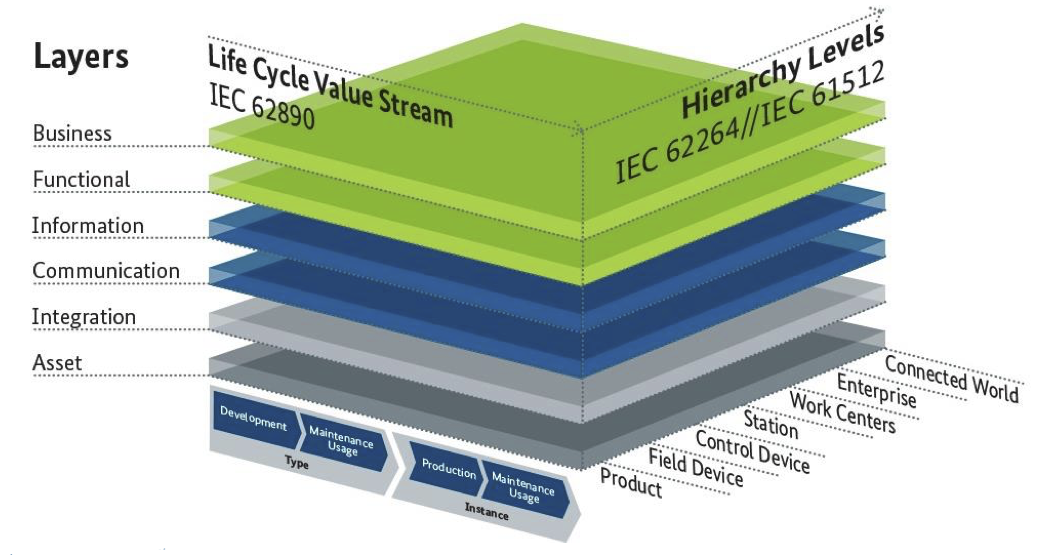
\includegraphics[width=15cm]{rami40}
  \caption{RAMI 4.0 - \cite{rami2016}}
  \label{Kap2:RAMI 4.0}
\end{figure}

\clearpage

Jeder Teilnehmer der Architektur wird als Asset bezeichnet und besitzt seine eigene Verwaltungsschale, welche als Schnittstelle zum Austausch von Informationen dient. Die Verwaltungsschale ist der Übergang zwischen der physischen zur digitalen Welt.

TODO - genauer auf die einzelnen Komponenten eingehen? Notwendig?
TODO - siehe DIN 91345
TODO - Anforderungen an diese Komponenten unterschiedlich

\section{sichere Kommunikation in Industrie 4.0}
Im Gegensatz zur I3.0, in welcher Daten auf lokaler Ebene oder zwischen einzelnen internen Unternehmensebenen ausgetauscht wurden, stellt in der I4.0 der Austausch von Daten und Informationen über Unternehmensgrenzen hinweg eine wesentliche Herausforderung dar. Dabei findet die Kommunikation nicht mehr über ein Enterprise-Resource-Planning-System (ERP) statt, sondern auch direkt von einer darunterliegenden Ebene, wie z. B. einer Maschine mit ihrem Lieferanten. Durch diese enge Vernetzung können sowohl Menschen, als auch Maschinen die Kommunikationspartner sein. Um diese Kommunikation sicher und zuverlässig zu gestalten, müssen die Grundprinzipien der sicheren Kommunikation realisiert werden.

\subsection{Grundprinzipien der sicheren Kommunikation}
\subsubsection{Vertraulichkeit/Zugriffsschutz}
\subsubsection{(Daten-)Integrität/Änderungsschutz}
\subsubsection{Authentizität/Fälschungsschutz}
\subsubsection{Verbindlichkeit/Nichtabstreitbarkeit}
\subsubsection{Anonymität}

Industrie 4.0 beinhaltet durch die Unternehmensübergreifende Kommunikation außerdem den rechtlichen Rahmen, welcher bei Nichteinhaltung von Verträgen bzgl. Verfügbarkeit, Integrität und Vertraulichkeit gelten kann.

\subsection{Anforderungen}
\subsection{Komponenten einer I4.0 Architektur}
\subsubsection{Assets}
\subsubsection{Smarte Sensoren}
\subsubsection{TODO}

\section{Kommunikationsstrukturen in Industrie 4.0 Umgebungen}
Um die Kommunikation zwischen verschiedenen Teilnehmern zu ermöglichen, ergeben sich in der Praxis unterschiedliche Strukturen. Jede dieser Strukturen bietet, je nach Anwendungsfall und zu erfüllenden Anforderungen, Vor- und Nachteile.

TODO - mehr -> siehe sichere Kommunikation-i4.0

\subsection{End2End}
Die Komponenten der Industrie 4.0 Umgebung kommunizieren über einen direkten Kanal miteinander. Dies setzt voraus, dass sich beide Teilnehmer in einem Netzwerk befinden, welches die benötigten Dienste wie z. B. \ac{IP} und \ac{DNS} zur Kommunikation bereitstellt. Des weiteren müssen beide Systeme diese Dienste und Protokolle unterstützen.

\subsection{Gateways}
Um existierende Systeme, welche selbst nicht Industrie 4.0 konform kommunizieren oder zu wenig Rechenleistung besitzen, in die Industrie 4.0 Welt zu integrieren, werden Industrie 4.0 Gateways genutzt. Dabei ist jedoch zu beachten, dass die Systeme hinter den Gateways nicht als Industrie 4.0 Komponenten entwickelt wurden und somit auch keine oder nur wenige dieser Eigenschaften besitzen. Des Weiteren ist es möglich, dass die Kommunikation aus Leistungsgründen oder besonderer Anforderungen über optimierte, proprietäre Protokolle stattfindet. Die Gateways müssen auf die Systeme und deren Protokolle individuell konfiguriert werden, um die Funktionalitäten im Industrie 4.0 Netz bereitstellen zu können, und die Kommunikation zu schützen.

TODO - Trumpf

\subsection{Publish-Subscribe}
Das Publish-Subscribe Modell bietet die Möglichkeit Informationen an mehrere Teilnehmer zu verteilen. Hierbei melden sich die Empfänger beim Verteiler an und wählen aus, über welche Nachrichtentypen sie informiert werden möchten. Diese Verteilservices nutzen zur besseren Skalierung und Reduzierung der Netzlast häufig Datagramme wie \ac{UDP}. Durch die Nutzung von Datagrammen geht jedoch die Fehlertoleranz verloren. Somit muss entweder dafür gesorgt werden, dass eine sehr zuverlässige Netzwerkinfrastruktur vorhanden ist und hohe Bandbreitenreserven geschaffen werden, um die Dienstgüte (\ac{QoS}) sicherzustellen oder dieses Modell nur für fehlertolerante Kommunikation wie z. B. Audio- und Video-Anwendungen oder Businessprozesse zu nutzen. 

\subsection{Kommunikation mit Netzwerk als Partner}
Zeitkritische Automatisierungsanwendungen verlangen besondere Netzwerkeigenschaften. Sie können auf Latenz oder Jitter angewiesen sein. Um diese Eigenschaften sicherzustellen, ist es sinnvoll in diese Netze eine Industrie 4.0 Schnittstelle zu integrieren. Somit ist es den Teilnehmern möglich, über die Verwaltungsschale sicherzustellen, dass das Netzwerk die erforderlichen Anforderungen bereitstellt. \cite{sichKom2017}

TODO - Bilder undso -> sichere-kommunikation-i40